%_______________________________________________________________________________
% main.tex

\input{preamble12.tex}
\hypersetup{%
    pdfauthor={Mike Pierce}%
   ,pdftitle={Pop Quiz | Math 113}%
   ,pdfkeywords={Pierce,CMU,Colorado,College Algebra,113}%
   ,pageanchor=false%
}
\geometry{
    margin=1in%
   ,left=0.75in%
   ,right=0.75in%
}
\usepackage{fourier}
\usepackage[default]{comicneue}
\input{accessible-colors.tex}
\input{newcommand.tex}
\input{newenvironment.tex}
\pagenumbering{gobble}
\usepackage{pagegrid}
\pagegridsetup{
    step=0.5in
    ,firstcolor=blue
    ,secondcolor=orange
    ,foreground=true
    ,disable
}


\begin{document}

\begin{center}
    {\Huge{Pop Quiz}}
    \\ Math 113-001/6 College Algebra
    \\ Colorado Mesa University Fall 2022
\end{center}

\vspace{0.5in-2px}
%\vspace{2em}
%\textsc{Name}: \enspace \hrulefill
%\vspace{1em}

\begin{enumerate}

    \item 
        How can you find all the roots of
        the polynomial \( x^4-7x^3+12x^2 \)
        without using technology?
        \vfill\null

    \item 
        How can you find all the roots of
        the polynomial \( x^4-7x^2+12 \)
        without using technology?
        \vfill\null

    \item 
        What is an equation of the unique degree-four polynomial
        whose graph passes through all of these points?
        \[ (1,-3) \qquad (2,2) \qquad (3,5) \qquad (4,3) \qquad (5,1) \]
        \vfill\null

        \newpage

    %\item 
    %    What are all the solutions to the equation
    %    \[ \frac{x^2+8}{x+2} = -12 \,?  \]
    %    \vfill\null

    \item 
        What degree might the polynomial whose graph is below have?
        \par\begin{figure}[h]
            \centering 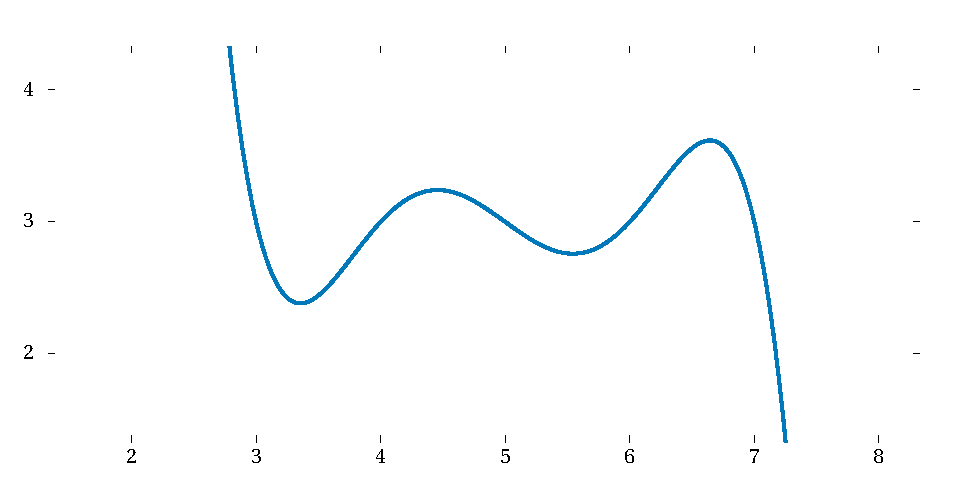
\includegraphics[width=0.83\textwidth]{figures/poly/main.pdf}
        \end{figure}

    \item 
        How can you find all the roots of
        the polynomial \( x^3-x^2-8x+12\)
        without using technology,
        if you know one of the roots is \(2\)?
        \vfill\null
        \vfill\null

    \item 
        Fifty counting numbers (positive whole numbers) are written down in a list
        in such a way so that the sum of any four consecutive numbers is \(53\). 
    The first number is \(3\), the 19th number is eight times the 13th number, 
    and the 28th number is five times the 37th number. What is the 44th number?

\end{enumerate}

\end{document}

